% =====================================================================
% Feedback-Augmented RT-DETR — Beamer presentation
% Hatem Saadallah & Nour Jennane — Bocconi CV — April 2026
%
% Build:
%   cd presentation/beamer && make
% Or directly:
%   pdflatex main.tex && pdflatex main.tex
% =====================================================================
\documentclass[aspectratio=169,11pt]{beamer}

\usetheme[progressbar=frametitle, sectionpage=progressbar,
          numbering=fraction, block=fill]{metropolis}

\usepackage[utf8]{inputenc}
\usepackage[T1]{fontenc}
\usepackage{amsmath, amssymb, mathtools}
\usepackage{tikz}
\usetikzlibrary{positioning, arrows.meta, shapes.geometric, calc, fit}
\usepackage{booktabs}
\usepackage{graphicx}
\usepackage{xcolor}

% --- palette ---
\definecolor{Navy}{HTML}{1F6FEB}
\definecolor{Dark}{HTML}{1A1A2E}
\definecolor{Light}{HTML}{66667A}
\definecolor{GoodGreen}{HTML}{2CA02C}
\definecolor{BadRed}{HTML}{D62C2E}
\definecolor{LightBlueBg}{HTML}{F0F6FF}
\definecolor{LightGreenBg}{HTML}{E8F7E8}
\definecolor{LightRedBg}{HTML}{FDECEC}

% metropolis colors — match the pptx version
\setbeamercolor{normal text}{fg=Dark, bg=white}
\setbeamercolor{alerted text}{fg=BadRed}
\setbeamercolor{example text}{fg=GoodGreen}
\setbeamercolor{title}{fg=Dark}
\setbeamercolor{frametitle}{fg=white, bg=Navy}
\setbeamercolor{progress bar}{fg=Navy, bg=Light!30}
\setbeamercolor{block title}{fg=white, bg=Navy}
\setbeamercolor{block body}{bg=LightBlueBg}

% --- figure paths ---
\graphicspath{
    {../_build/}
    {../../report/figures/}
}

% --- title ---
\title{Feedback-Augmented RT-DETR}
\subtitle{for Small Object Detection}
\author{Hatem Saadallah \and Nour Jennane}
\institute{Computer Vision and Image Processing\\Bocconi University}
\date{Final Project — April 2026}

% --- helpers ---
% A "spotlight" command that draws a thick colored ellipse, used inside
% \only<2-> blocks to reveal an annotation on the second click.
\newcommand{\spotlight}[5][GoodGreen]{%
    % args: [color], width, height, x-shift, y-shift (relative to current cursor)
    \begin{tikzpicture}[remember picture, overlay]
        \draw[#1, line width=1.4mm] ($(current page.center)+(#4,#5)$)
            ellipse [x radius=#2, y radius=#3];
    \end{tikzpicture}%
}

\begin{document}

% =====================================================================
% TITLE
% =====================================================================
\maketitle

% =====================================================================
% SECTION 1 — PROBLEM FORMULATION
% =====================================================================
\section{Problem Formulation}

\begin{frame}{Small objects are harder to detect}
    \begin{columns}[T, onlytextwidth]
        \column{0.55\textwidth}
        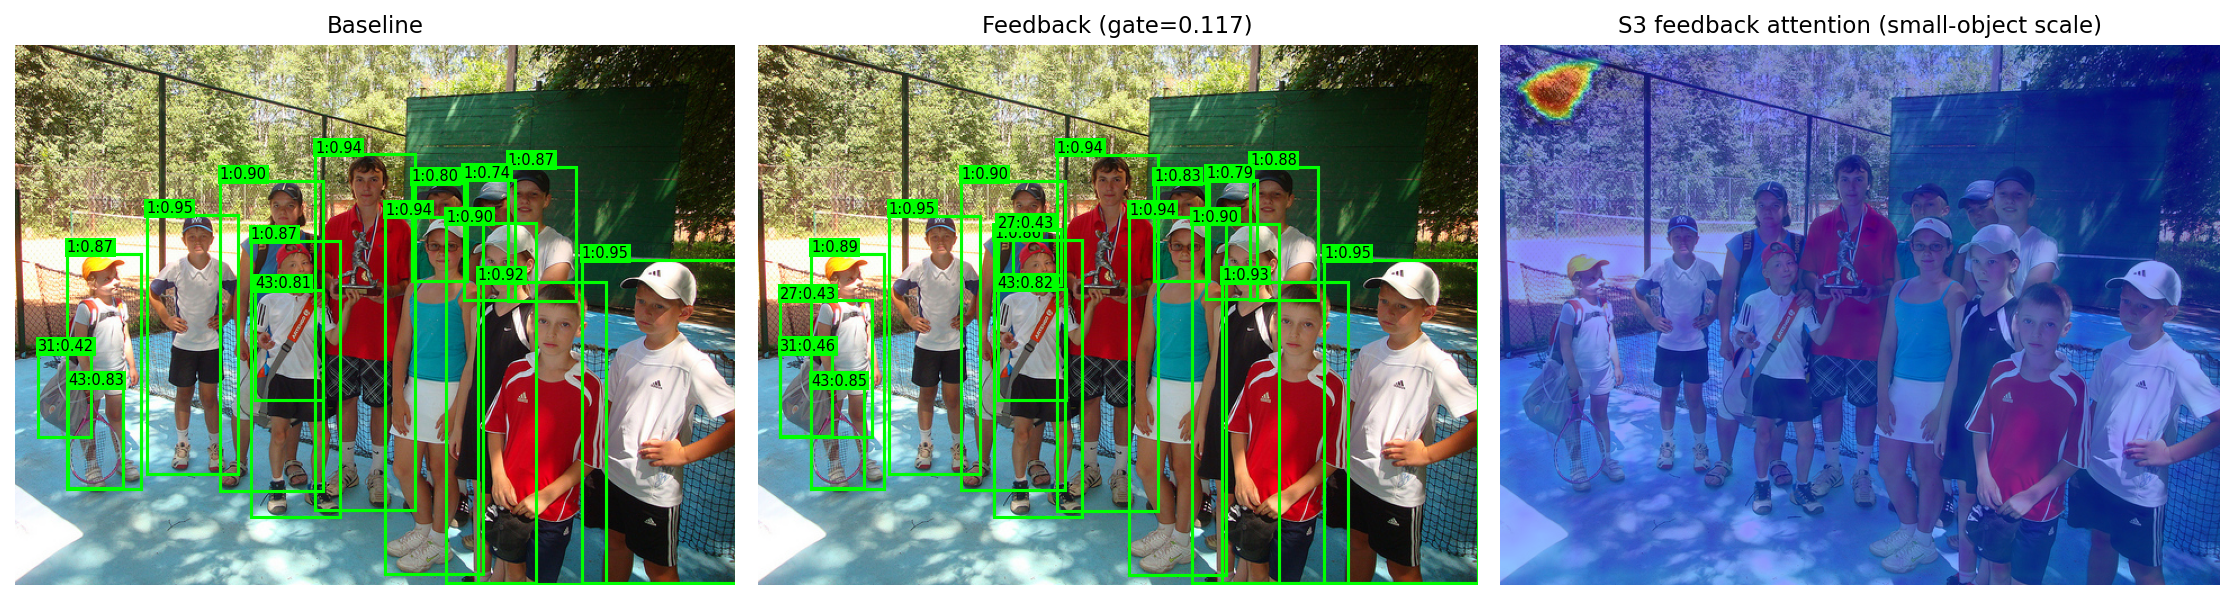
\includegraphics[width=\linewidth]{viz_000000001000.png}

        \column{0.4\textwidth}
        \vspace{0.5em}
        {\small\color{Light}AP\textsubscript{L} (large)}\\[0.2em]
        {\fontsize{60}{60}\selectfont\bfseries\color{GoodGreen}67.7}

        \vspace{1em}
        {\small\color{Light}AP\textsubscript{S} (small)}\\[0.2em]
        {\fontsize{60}{60}\selectfont\bfseries\color{BadRed}34.7}

        \vspace{1em}
        \emph{33-point gap. Why?}
    \end{columns}
\end{frame}

\begin{frame}{RT-DETR: backbone $\rightarrow$ encoder $\rightarrow$ decoder}
    \centering
    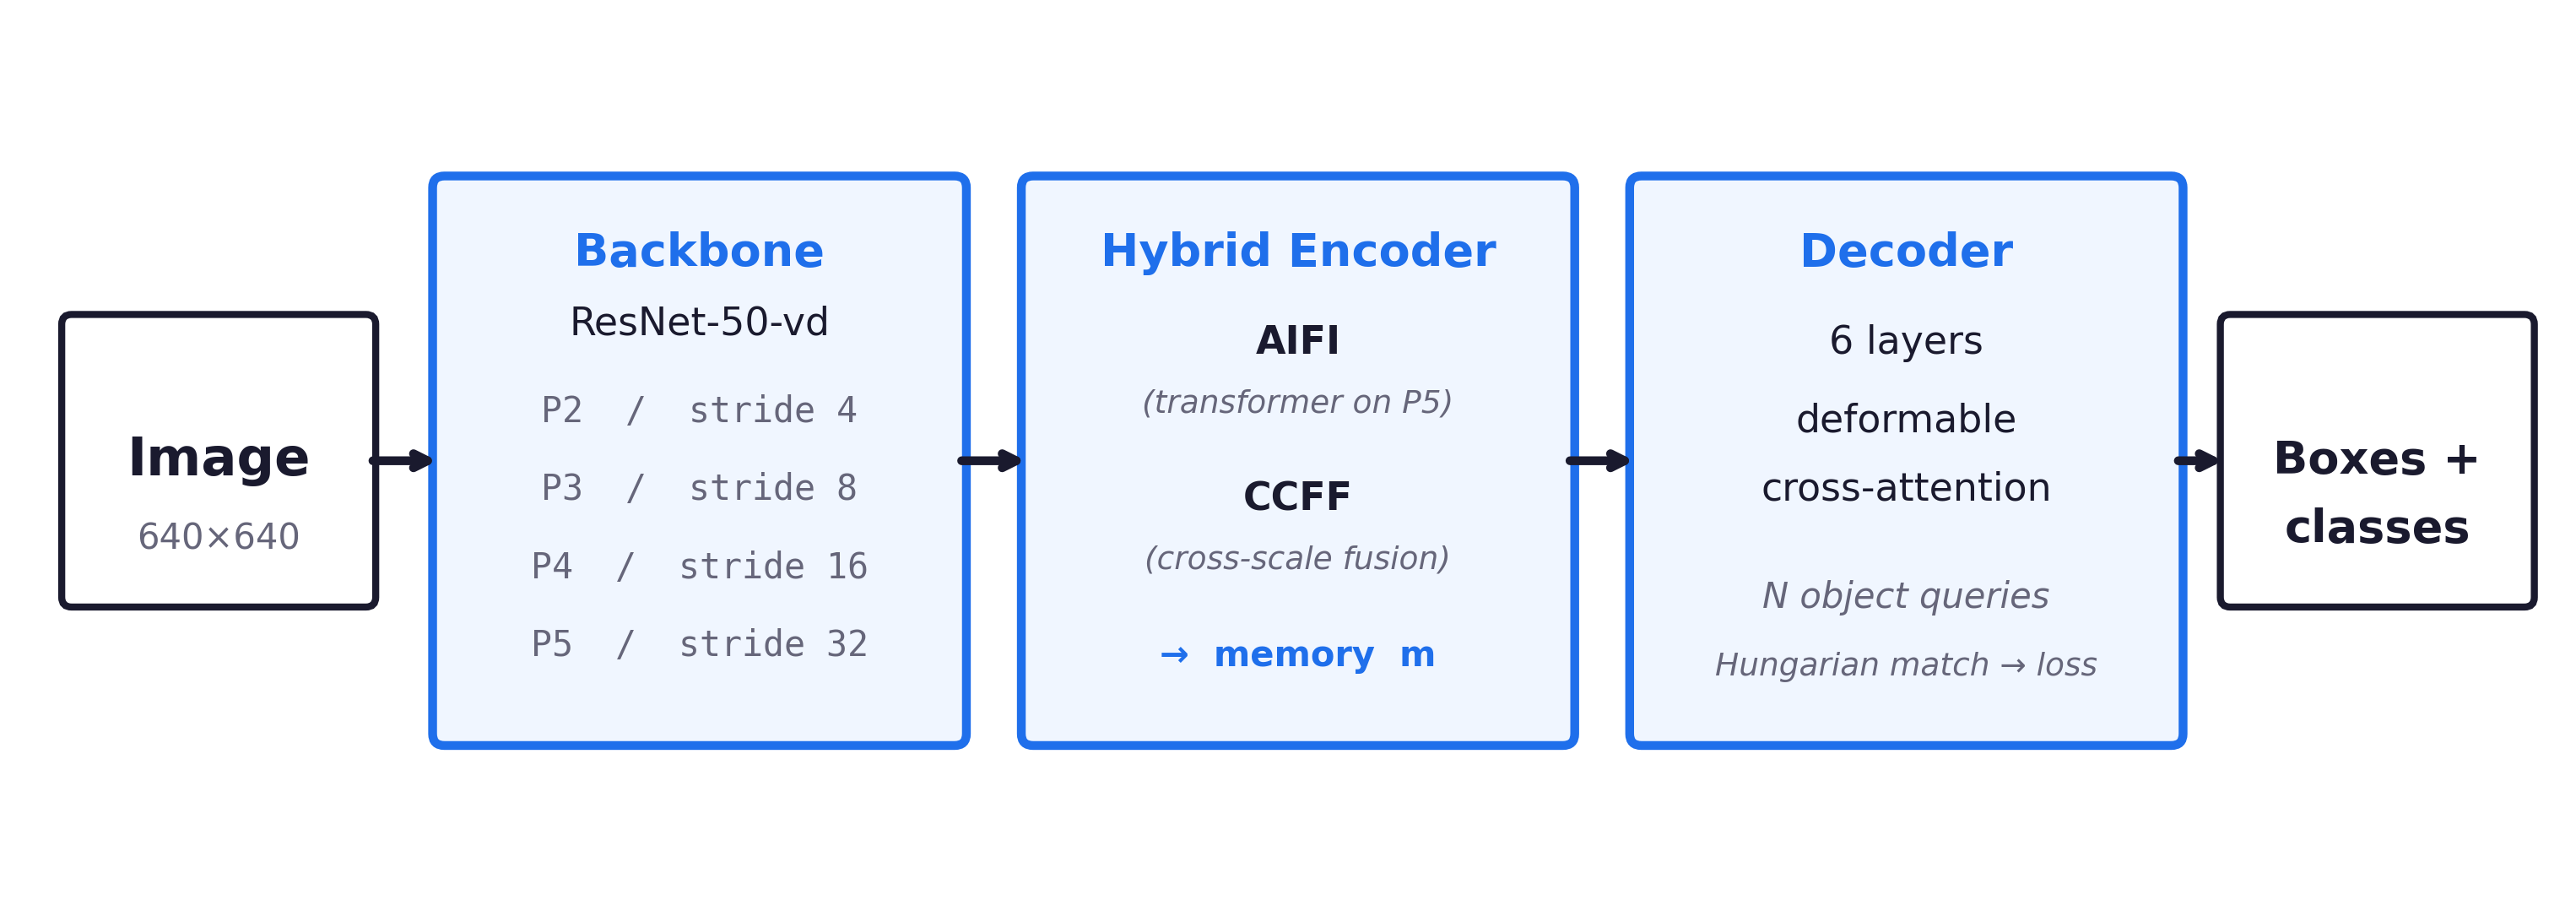
\includegraphics[width=0.95\linewidth]{diag_rtdetr.png}
    \vspace{0.5em}

    \small End-to-end, NMS-free. Six decoder layers all attend over
    the same encoder memory.
\end{frame}

\begin{frame}{The reason is structural}
    \centering
    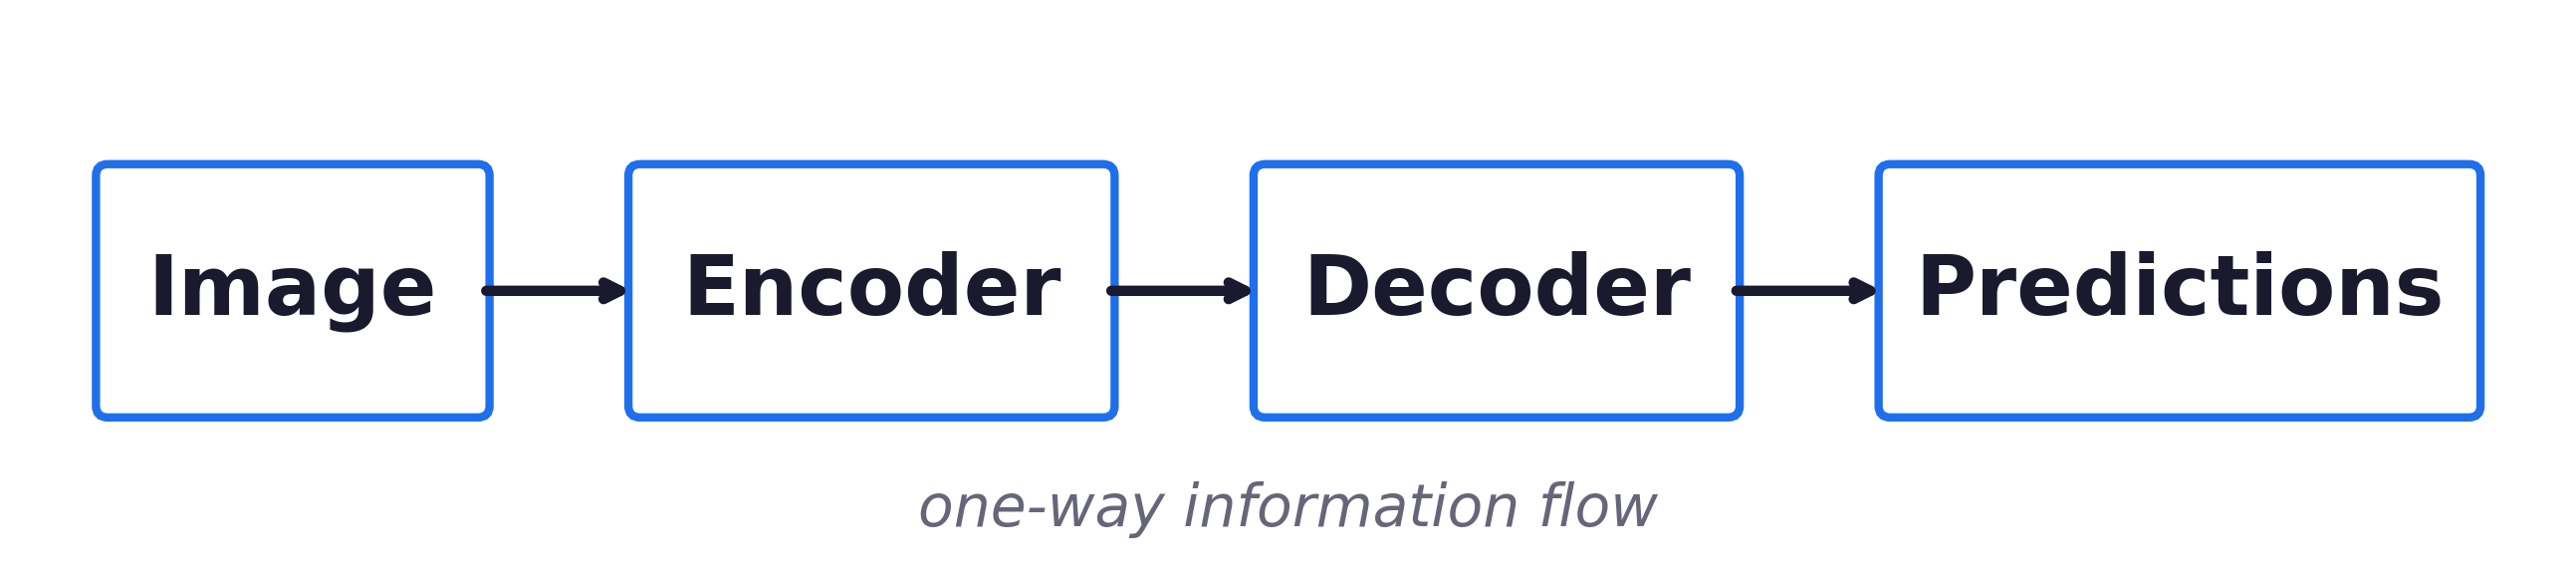
\includegraphics[width=0.85\linewidth]{diag_baseline.png}
    \vspace{1em}

    Encoder memory is computed once. The decoder cannot revise it.

    \vspace{0.5em}
    {\small\color{Light}\itshape
    Refinement of the features small objects live in is a one-way street.}
\end{frame}

% =====================================================================
% SECTION 2 — DATA SOURCING STRATEGY
% =====================================================================
\section{Data Sourcing Strategy}

\begin{frame}{COCO 2017 — the standard small-object benchmark}
    \begin{columns}[T]
        \column{0.5\textwidth}
        \begin{block}{Dataset}
            \textbf{Microsoft COCO 2017}

            \vspace{0.5em}
            \textbf{Splits}\\
            \texttt{train2017} — 118k images, 860k boxes\\
            \texttt{val2017}\hphantom{xx} — 5k images (held out)

            \vspace{0.5em}
            \textbf{Pre-trained weights}\\
            {\small\texttt{rtdetr\_r50vd\_6x\_coco.pth}\\(public, finetuned 13 ep)}
        \end{block}

        \column{0.5\textwidth}
        \begin{block}{Why COCO?}
            \begin{itemize}\setlength\itemsep{0.4em}
                \item Standard benchmark — directly comparable to
                      RT-DETR, DETR, YOLO.
                \item Has explicit small / medium / large size buckets
                      (AP\textsubscript{S} / AP\textsubscript{M} / AP\textsubscript{L}).
                \item ${\sim}41\%$ of annotated boxes are small (area $< 32^{2}$ px).
                \item Same pre-training corpus as our baseline $\to$ fair comparison.
            \end{itemize}
        \end{block}
    \end{columns}
\end{frame}

% =====================================================================
% SECTION 3 — PROPOSED SOLUTION
% =====================================================================
\section{Proposed Solution}

\begin{frame}{Our idea: let the model refine its own features}
    \centering
    
\includegraphics[width=0.85\linewidth]{diag_idea.png}

    \vspace{1em}
    Feed early decoder predictions back into the encoder memory.
\end{frame}

% --- MATH 1: Attention ---
\begin{frame}{Attention, in one line}
    \vspace{0.6em}
    \begin{equation*}
        \mathrm{Attn}(\mathbf{Q}, \mathbf{K}, \mathbf{V}) \;=\;
        \mathrm{softmax}\!\left(\frac{\mathbf{Q}\,\mathbf{K}^{\top}}
        {\sqrt{d}}\right)\mathbf{V}
    \end{equation*}

    \vspace{1em}
    \begin{columns}[T, onlytextwidth]
        \column{0.33\textwidth}
        \centering
        {\fontsize{40}{40}\selectfont\bfseries\color{Navy}Q}\\[0.4em]
        what we look for\\
        {\small\itshape\color{Light}(query)}

        \column{0.33\textwidth}
        \centering
        {\fontsize{40}{40}\selectfont\bfseries\color{orange!90!black}K}\\[0.4em]
        where we look\\
        {\small\itshape\color{Light}(addresses)}

        \column{0.33\textwidth}
        \centering
        {\fontsize{40}{40}\selectfont\bfseries\color{GoodGreen}V}\\[0.4em]
        what we extract\\
        {\small\itshape\color{Light}(contents)}
    \end{columns}

    \vfill
    {\small\itshape\color{Light}\centering
    Attention lets the model focus on important parts of the image.\par}
\end{frame}

% --- MATH 2: Feedback rule ---
\begin{frame}{Our feedback rule}
    \vspace{0.6em}
    \begin{equation*}
        \mathbf{m}' \;=\; \mathbf{m} \;+\; g \cdot
        \mathrm{Attn}(\mathbf{m},\, \mathbf{t})
    \end{equation*}

    \vspace{1em}
    \begin{columns}[T, onlytextwidth]
        \column{0.33\textwidth}
        \centering
        {\fontsize{40}{40}\selectfont\bfseries\color{Navy}m}\\[0.4em]
        encoder memory\\
        {\small\itshape\color{Light}(image features)}

        \column{0.33\textwidth}
        \centering
        {\fontsize{40}{40}\selectfont\bfseries\color{orange!90!black}g}\\[0.4em]
        gate\\
        {\small\itshape\color{Light}(how much feedback)}

        \column{0.33\textwidth}
        \centering
        {\fontsize{40}{40}\selectfont\bfseries\color{GoodGreen}t}\\[0.4em]
        decoder output\\
        {\small\itshape\color{Light}(early predictions)}
    \end{columns}

    \vfill
    {\small\itshape\color{Light}\centering
    We update the encoder using the decoder's own predictions.\par}
\end{frame}

% --- v1 first attempt + spotlight (single frame, 2 clicks) ---
\begin{frame}{First attempt (v1) — and why it failed}
    \begin{center}
    \emph{Plain sigmoid gate, applied to all four pyramid levels.}
    \end{center}
    \vspace{0.5em}

    \begin{columns}[c, onlytextwidth]
        \column{0.55\textwidth}
        \centering
        
\begin{tikzpicture}
            \node[font=\fontsize{44}{50}\selectfont\bfseries,
                  color=BadRed] (val) {$\Delta\mathrm{AP}_S \;=\; 0.00$};
            % Spotlight on second click: red oval around the 0.00
            \only<2->{
                \draw[BadRed, line width=1.2mm]
                    ($(val.east)+(-1.2,0)$) ellipse [x radius=1.0, y radius=0.65];
            }
        \end{tikzpicture}\\[1em]
        {\small\itshape\color{Light}the mechanism contributed nothing}

        \column{0.4\textwidth}
        \textbf{Why?}

        \vspace{0.5em}
        $\alpha$ drifts to $-\infty\;\to\;$ gate ${\approx}\,0.$

        \vspace{0.6em}
        The feedback signal is multiplied by zero before reaching memory.
    \end{columns}
\end{frame}

% --- v2 fixes ---
\begin{frame}{v2: two fixes — zero new parameters}
    \centering
    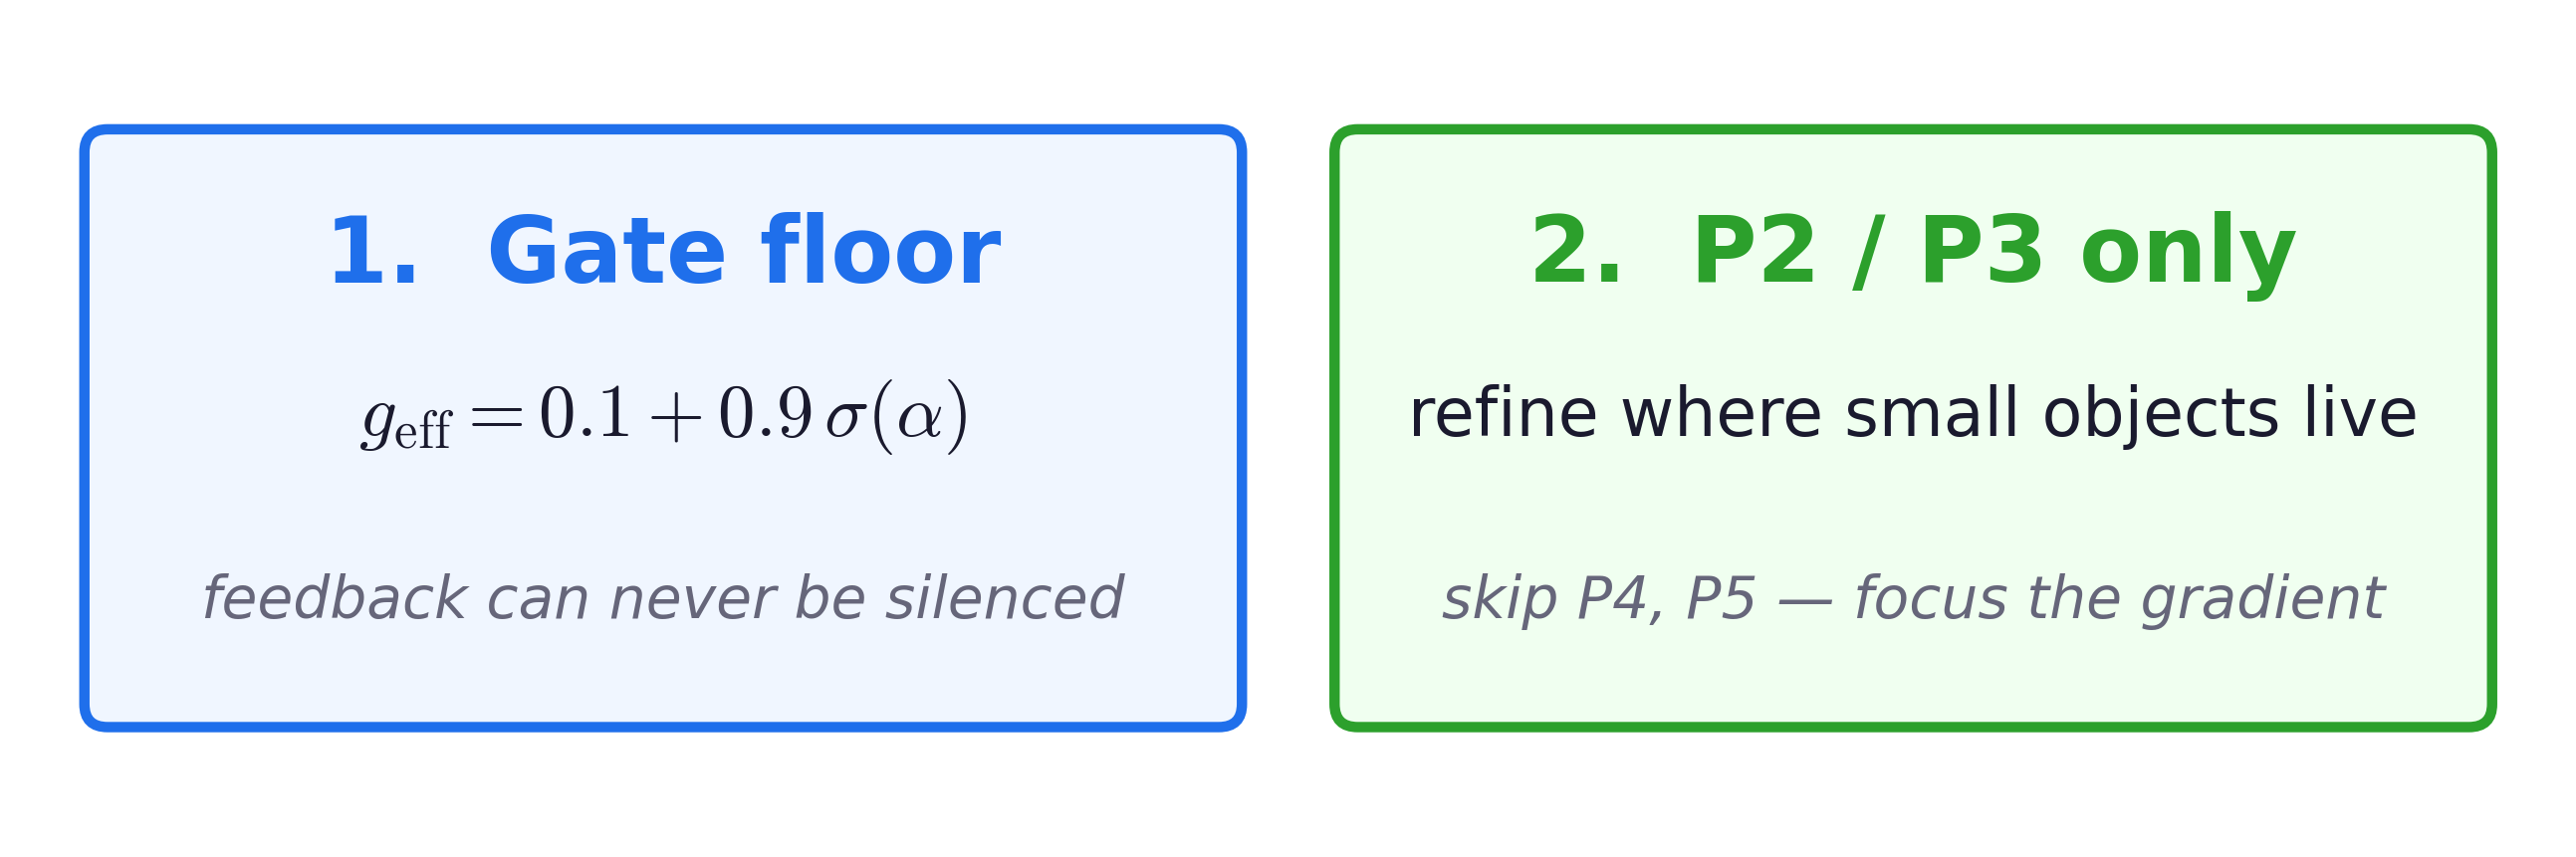
\includegraphics[width=0.95\linewidth]{diag_v2_fixes.png}

    \vspace{0.8em}
    {\small\itshape\color{Light}
    Reparameterize the gate. Refine only the levels small objects live in.}
\end{frame}

% =====================================================================
% SECTION 4 — EVALUATION APPROACH
% =====================================================================
\section{Performance Evaluation Approach}

\begin{frame}{How we evaluate the contribution}
    \begin{columns}[T]
        \column{0.5\textwidth}
        \begin{block}{Metrics (COCO standard)}
            \footnotesize
            AP, AP\textsubscript{S}, AP\textsubscript{M}, AP\textsubscript{L}
            — IoU 0.5..0.95\\[0.3em]
            \textbf{AP\textsubscript{S} is the headline metric}
            (area $<32^2$ px)
        \end{block}

        \column{0.5\textwidth}
        \begin{block}{Baselines}
            \footnotesize
            \begin{itemize}\setlength\itemsep{0.1em}
                \item RT-DETR-R50 (published)
                \item v1 feedback (before the fix)
                \item \textbf{v2 feedback} (with the fix)
            \end{itemize}
        \end{block}
    \end{columns}

    \begin{center}
    \textcolor{Navy}{\textbf{Same-checkpoint ablation — isolates causal contribution}}\\[0.3em]
    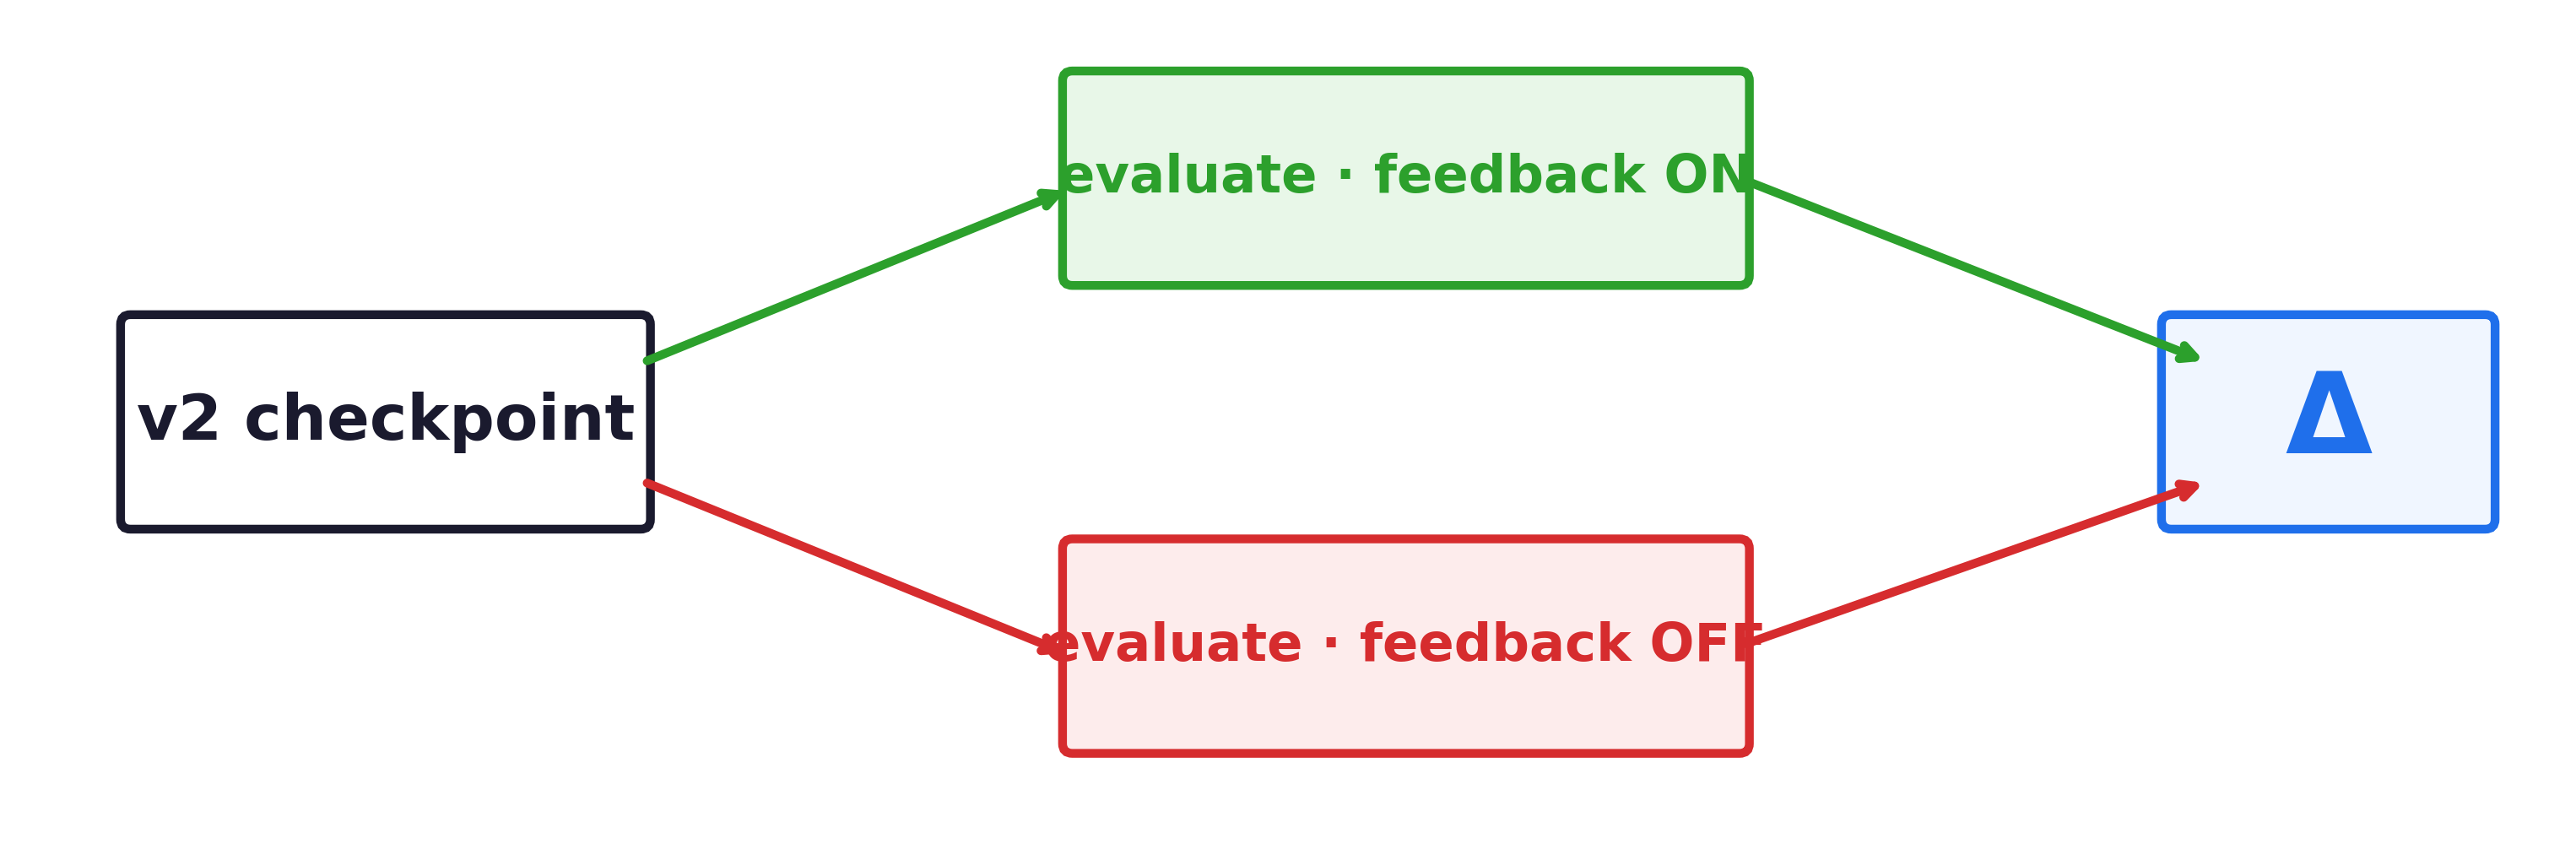
\includegraphics[width=0.65\linewidth]{diag_ablation.png}\\[0.2em]
    {\footnotesize\itshape\color{Light}
    Toggle feedback ON / OFF at inference. Identical weights, identical inputs.}
    \end{center}
\end{frame}

% =====================================================================
% SECTION 5 — FINAL RESULTS
% =====================================================================
\section{Final Results}

% --- Training trajectory + spotlight on the crossover ---
\begin{frame}{Training: v2 climbs faster, ends higher}
    \centering
    \begin{tikzpicture}
        \node[anchor=center] (img) {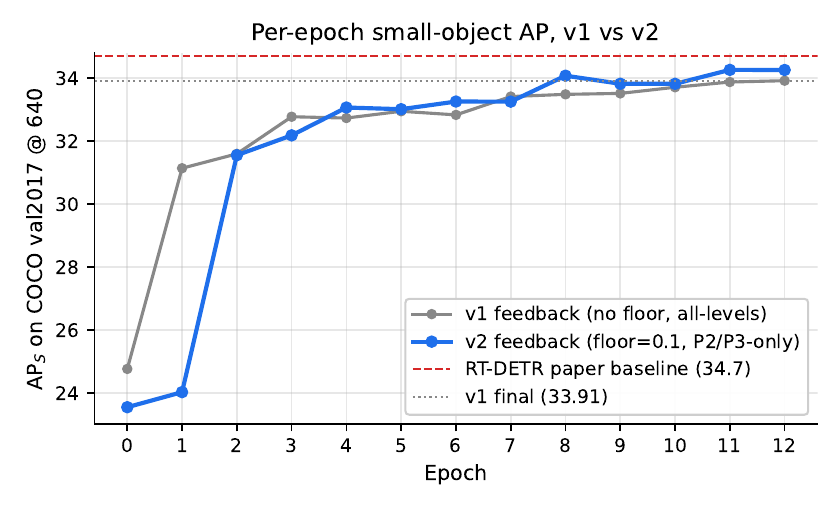
\includegraphics[width=0.78\linewidth]{learning_curves.png}};
        % Spotlight on second click: green circle on the v2 crossover
        \only<2->{
            \draw[GoodGreen, line width=1.2mm]
                ($(img.center)+(1.45, 1.55)$) ellipse [x radius=0.45, y radius=0.32];
            \node[anchor=west, color=GoodGreen, font=\bfseries, font=\small]
                at ($(img.center)+(2.0, 1.05)$) {v2 crosses here};
            \node[anchor=west, color=GoodGreen, font=\itshape\footnotesize]
                at ($(img.center)+(2.0, 0.7)$) {at epoch 8 (4 early)};
        }
    \end{tikzpicture}

    \vspace{0.4em}
    {\footnotesize\itshape\color{Light}
    v2 first crosses v1's final 33.91 at epoch 8 — four epochs early.}
\end{frame}

% --- Final scores ---
\begin{frame}{Final performance (with feedback ON)}
    \begin{columns}[c, onlytextwidth]
        \column{0.5\textwidth}
        \begin{center}
        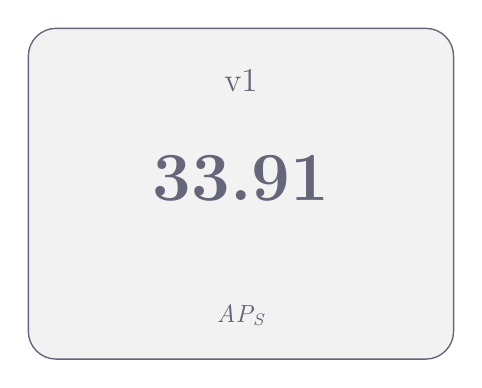
\begin{tikzpicture}
            \node[draw=Light, line width=0.5pt, rounded corners=10pt,
                  fill=gray!10, minimum width=5.4cm, minimum height=4.2cm] {};
            \node[anchor=north, font=\large\color{Light}]
                at (0, 1.7) {v1};
            \node[font=\fontsize{44}{44}\selectfont\bfseries\color{Light}]
                at (0, 0.2) {33.91};
            \node[anchor=south, font=\itshape\small\color{Light}]
                at (0, -1.8) {AP\textsubscript{S}};
        \end{tikzpicture}
        \end{center}

        \column{0.5\textwidth}
        \begin{center}
        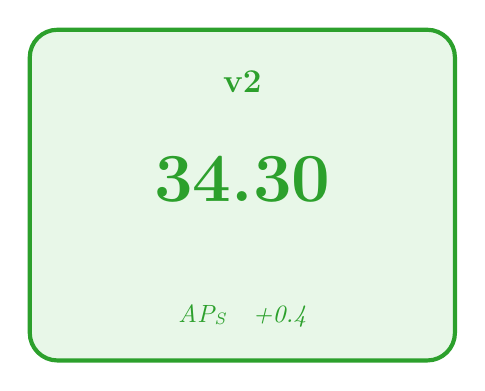
\begin{tikzpicture}
            \node[draw=GoodGreen, line width=1.5pt, rounded corners=10pt,
                  fill=LightGreenBg, minimum width=5.4cm, minimum height=4.2cm] {};
            \node[anchor=north, font=\large\bfseries\color{GoodGreen}]
                at (0, 1.7) {v2};
            \node[font=\fontsize{44}{44}\selectfont\bfseries\color{GoodGreen}]
                at (0, 0.2) {34.30};
            \node[anchor=south, font=\itshape\small\color{GoodGreen}]
                at (0, -1.8) {AP\textsubscript{S}\quad +0.4};
        \end{tikzpicture}
        \end{center}
    \end{columns}
\end{frame}

% --- Causal effect + spotlight on +0.99 ---
\begin{frame}{Causal effect of feedback}
    \vspace{0.5em}
    \begin{columns}[c, onlytextwidth]
        \column{0.30\textwidth}
        \centering
        {\large\color{Light}ON}\\[0.3em]
        {\fontsize{40}{40}\selectfont\bfseries\color{GoodGreen}34.25}\\[0.5em]
        {\itshape\small\color{Light}feedback enabled}

        \column{0.30\textwidth}
        \centering
        {\large\color{Light}OFF}\\[0.3em]
        {\fontsize{40}{40}\selectfont\bfseries\color{Light}33.26}\\[0.5em]
        {\itshape\small\color{Light}feedback bypassed}

        \column{0.30\textwidth}
        \centering
        {\large\color{Light}$\Delta$}\\[0.3em]
        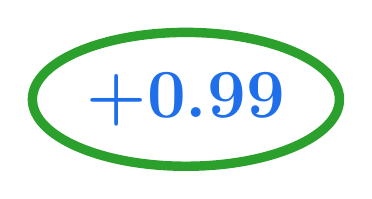
\begin{tikzpicture}
            \node[font=\fontsize{40}{40}\selectfont\bfseries\color{Navy}] (d)
                {+0.99};
            \only<2->{
                \draw[GoodGreen, line width=1.2mm]
                    (d.center) ellipse [x radius=1.95, y radius=0.85];
            }
        \end{tikzpicture}\\[0.5em]
        {\itshape\small\color{Light}the contribution}
    \end{columns}

    \vspace{1.5em}
    \begin{center}
    \textbf{\color{Navy}Feedback has a real causal impact on small-object detection.}
    \end{center}
\end{frame}

% --- Higher resolution + spotlight on 37.01 ---
\begin{frame}{Higher resolution $\to$ bigger gain}
    \vspace{1em}
    \begin{columns}[c, onlytextwidth]
        \column{0.45\textwidth}
        \centering
        {\large\color{Light}640 $\times$ 640}\\[0.5em]
        {\fontsize{42}{42}\selectfont\bfseries\color{Dark}34.25}

        \column{0.10\textwidth}
        \centering
        
\begin{tikzpicture}
            \draw[Navy, line width=1.6mm, -{Latex[length=4mm,width=4mm]}]
                (0, 0) -- (1.0, 0);
        \end{tikzpicture}

        \column{0.45\textwidth}
        \centering
        {\large\bfseries\color{Navy}800 $\times$ 800}\\[0.5em]
        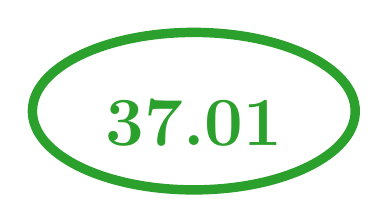
\begin{tikzpicture}
            \node[font=\fontsize{42}{42}\selectfont\bfseries\color{GoodGreen}] (v)
                {37.01};
            \only<2->{
                \draw[GoodGreen, line width=1.2mm]
                    ($(v.center)+(0, 0.15)$) ellipse [x radius=2.05, y radius=1.0];
            }
        \end{tikzpicture}
    \end{columns}

    \vspace{2.5em}
    \begin{center}
    \emph{+2.76 from more pixels.}\\[0.4em]
    {\small\color{Light}Feedback helps. Spatial sampling helps too.}
    \end{center}
\end{frame}

% --- Strengths + Limitations ---
\begin{frame}{Strengths and limitations}
    \begin{columns}[T]
        \column{0.5\textwidth}
        \begin{block}{\color{white}\textbf{+}\hspace{0.5em}Strengths}
            \begin{itemize}\setlength\itemsep{0.3em}
                \item Causal contribution: \textbf{+0.99} on small-object AP, same checkpoint.
                \item Zero new parameters relative to v1.
                \item Consistent improvement on every metric (AP, S, M, L).
                \item Robust at higher resolution (37.01 small-object AP at $800{\times}800$).
            \end{itemize}
        \end{block}

        \column{0.5\textwidth}
        \setbeamercolor{block title}{fg=white, bg=BadRed}
        \setbeamercolor{block body}{bg=LightRedBg}
        \begin{block}{\color{white}\textbf{$-$}\hspace{0.5em}Limitations}
            \begin{itemize}\setlength\itemsep{0.3em}
                \item Single seed — multi-seed variance unmeasured.
                \item 13-epoch finetune (vs 72-epoch from scratch).
                \item Floor and mask not isolated (a $2{\times}2$ ablation is missing).
                \item ${\approx}2{\times}$ slower than baseline (53 $\to$ 26 FPS) — cost is the P2 level.
            \end{itemize}
        \end{block}
    \end{columns}
\end{frame}

% --- Future work: recovering FPS ---
\begin{frame}{Future work: recovering inference speed}
    \begin{center}
    \emph{The 2$\times$ slowdown comes from the P2 level, not the feedback module.}
    \end{center}
    \vspace{0.5em}

    \begin{columns}[T, onlytextwidth]
        \column{0.32\textwidth}
        \begin{block}{\textbf{1.}\hspace{0.5em}Train with P2, infer without}
            {\color{Navy}\small\itshape\textbf{fastest path}}\\[0.6em]
            \textbf{How.} Use P2 during training, remove it at inference.\\[0.6em]
            \textbf{\color{GoodGreen}Goal.} Keep most of the +0.99 gain without the P2 cost.
        \end{block}

        \column{0.32\textwidth}
        \begin{block}{\textbf{2.}\hspace{0.5em}Lighter P2 path}
            {\color{Navy}\small\itshape\textbf{compromise}}\\[0.6em]
            \textbf{How.} Reduce P2's cost — fewer channels or simpler projection.\\[0.6em]
            \textbf{\color{GoodGreen}Goal.} Preserve gains while reducing the high-resolution slowdown.
        \end{block}

        \column{0.32\textwidth}
        \begin{block}{\textbf{3.}\hspace{0.5em}Knowledge distillation}
            {\color{Navy}\small\itshape\textbf{principled}}\\[0.6em]
            \textbf{How.} Distil v2's gains into a faster baseline RT-DETR student.\\[0.6em]
            \textbf{\color{GoodGreen}Goal.} Recover baseline speed while keeping the AP\textsubscript{S} gains.
        \end{block}
    \end{columns}

    \vspace{0.4em}
    \begin{center}
    {\bfseries\color{Navy}\footnotesize
    Common goal: keep the +0.99 gain while approaching the 53 FPS baseline.}
    \end{center}
\end{frame}

% --- Conclusion ---
\begin{frame}{Conclusion}
    \begin{enumerate}\setlength\itemsep{1em}
        \item \textbf{Feedback improves small-object detection.}\\
              {\itshape\color{Light}+0.99 small-object AP, causal contribution at inference.}

        \item \textbf{Only works with proper design.}\\
              {\itshape\color{Light}Floor the gate; restrict to small-object levels.}

        \item \textbf{Modest but real.}\\
              {\itshape\color{Light}Consistent across metrics; reproducible from the same checkpoint.}
    \end{enumerate}
\end{frame}

% --- Thank you ---
\begin{frame}[plain]
    \vspace*{1.5cm}
    \begin{center}
        {\fontsize{56}{56}\selectfont\bfseries Thank you.}

        \vspace{1em}
        {\Large\color{Navy}Questions?}

        \vspace{2.5em}
        {\small Hatem Saadallah \quad$\cdot$\quad Nour Jennane}

        \vspace{0.5em}
        {\footnotesize\color{Light}\texttt{github.com/HatemSaadallah/feedback-augmented-rtdetr}}
    \end{center}
\end{frame}

\end{document}
